\documentclass[10pt]{beamer}
\usepackage{graphicx} % Required for inserting images
\usepackage{amssymb}
\usepackage{amsmath}
\usepackage{amsthm}
\usepackage{hyperref}
\usepackage{tikz} \usetikzlibrary{calc}
\usepackage{algpseudocode}
\usepackage{algorithm}
\usepackage{multirow}
\usepackage{tabularx}
\usepackage[table]{xcolor}
\usepackage{longtable}
\usepackage{subfigure}
\usepackage[most]{tcolorbox}
\usepackage{ulem}


\usetheme{Madrid}
\usecolortheme{seahorse}

\colorlet{myGray}{white!90!black}
\colorlet{myBlue}{blue!75!black}

\beamertemplatenavigationsymbolsempty
\setbeamertemplate{bibliography entry title}{}
\setbeamertemplate{bibliography entry location}{}
\setbeamertemplate{bibliography entry note}{}
\setbeamertemplate{bibliography item}{\insertbiblabel}
\setbeamercolor{bibliography item}{fg=black}
\setbeamercolor{bibliography entry author}{fg=black}
\setbeamercolor{bibliography entry title}{fg=black}
\setbeamercolor{bibliography entry location}{fg=black}
\setbeamercolor{bibliography entry note}{fg=black}
\setbeamertemplate{enumerate items}[default]

\newtcolorbox{mybox}{
    colback=white!95!black,
    frame hidden,
    enhanced jigsaw,
    breakable
    %fonttitle=\bfseries,
}

\newcommand{\code}[1]{\textcolor{myBlue}{\texttt{#1}}}

\title[PCCA]{\textbf{Modular integer arithmetic and SIMD vectorization using Intel AVX}}
\date{20 May 2025}
\author[D.ASSIRE, M.BONBOIRE]
{Damien ASSIRE \and Marie BONBOIRE}

\AtBeginSection[]
{
  \begin{frame}[noframenumbering]
    \frametitle{Table of Contents}
    \tableofcontents[currentsection, hideothersubsections]
  \end{frame}
}


\begin{document}

\begin{frame}[plain]
	\begin{center} 
		\includegraphics[scale=0.1]{su.png}
    \end{center}

    \titlepage
    
    \vfill
    \begin{flushleft}
        {\small
            \textbf{Supervisor:} Mr. Vincent NEIGER\footnote{\url{https://vincent.neiger.science/}} (LIP6 - PolSys)\\
        }
    \end{flushleft}
\end{frame}

\begin{frame}
    \frametitle{Table of Contents}
    \tableofcontents
\end{frame}

\section{Preface}
\begin{frame}
    \frametitle{Machines description}
    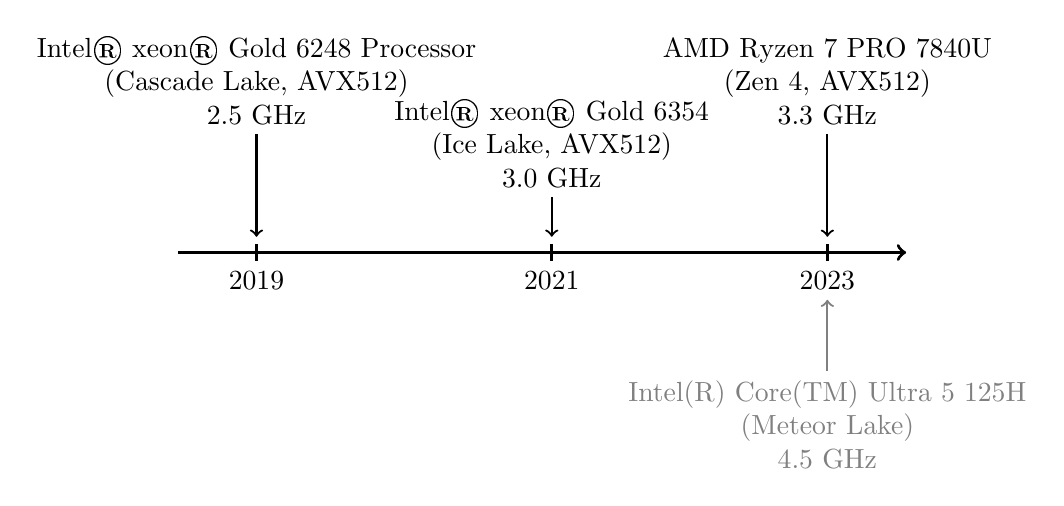
\begin{tikzpicture}[very thick, black]

        %coordinates
        \coordinate (O) at (0,0); % Origin
        \coordinate (F) at (9.25,0); %End
        \coordinate (P1) at (1,0); %ppti
        \coordinate (P2) at (4.75,0); %groebner
        \coordinate (P3) at (8.25,0); %mariz+argiope

        %proc
        \draw[<-,thick,color=black] ($(P1)+(0,0.2)$) -- ($(P1)+(0,1.5)$) node [above=0pt,align=center,black] 
        {Intel® xeon® Gold 6248 Processor \\ (Cascade Lake, AVX512) \\ 2.5 GHz};
        \draw[<-,thick,color=black] ($(P2)+(0,0.2)$) -- ($(P2)+(0,0.7)$) node [above=0pt,align=center,black] 
        {Intel® xeon® Gold 6354 \\ (Ice Lake, AVX512) \\ 3.0 GHz};
        \draw[<-,thick,color=black] ($(P3)+(0,0.2)$) -- ($(P3)+(0,1.5)$) node [above=0pt,align=center,black] 
        {AMD Ryzen 7 PRO 7840U \\ (Zen 4, AVX512) \\ 3.3 GHz};
        \draw[<-,thick,color=gray] ($(P3)-(0,0.6)$) -- ($(P3)-(0,1.5)$) node [below=0pt,align=center,gray] 
        {Intel(R) Core(TM) Ultra 5 125H \\ (Meteor Lake) \\ 4.5 GHz};

        %main arrow
        \draw[->] (O) -- (F);

        %ticks
        \foreach \x in {1,4.75,8.25}
        \draw(\x cm,3pt) -- (\x cm,-3pt);
        %labels
        \foreach \i \j in {1/2019,4.75/2021,8.25/2023}{
        	\draw (\i,0) node[below=3pt] {\j} ;
        }

\end{tikzpicture}
\end{frame}

\begin{frame}
    \begin{itemize}
        \item Vectorization
        \item Timings measurements
    \end{itemize}
\end{frame}

\section{Multiplication of 64-bit integers}
\subsection{Long multiplication}
\begin{frame}
    Long multiplication
\end{frame}

\subsection{Retrieve high and low part of the result}
\begin{frame}
    Low/high part of the result
\end{frame}

\subsection{Modular multiplication with a precomputation step}
\begin{frame}
    \frametitle{Modular multiplication with a precomputation step}

    \begin{example}
    Let $B$ be the maximum bitsize of a word ($B\in \{32, 64\}$). \\
    Given $n$ and $w \in \mathbb{Z}/n\mathbb{Z}$, one can compute a scaled approximation 
    of $\frac{w}{n}$, which is precisely $$ w_{pre} = \biggl\lfloor\dfrac{w\cdot 2^{B}}{n} \biggr\rfloor.$$
    \end{example}

    \bigskip
    For a vector $b = (b_1,\dots, b_N)$, one can compute 
    $$(w\cdot b_i \mod n) \text{ for each } i\in \{1, \dots, N\}$$

    using Shoup algorithm%\cite{Bos_Stam_2021}:

    \begin{enumerate}
        \item compute $p_{hi}, p_{lo}$ such that $w_{pre} \cdot b_i = p_{hi}\cdot 2^B + p_{lo}$, \hfill (1 \texttt{mulhi})
        \item compute $c = w\cdot b_i - p_{hi}\cdot n$, \hfill (2 \texttt{mullo})
        \item if $c \geq n$, return $c-n$, else return $c$ \\
            $\Longleftrightarrow \min(c-n, c)$.
    \end{enumerate}
\end{frame}

\section{Classic arithmetic operations on vectors}
\subsection{Addition of two vectors}
\begin{frame}
    Addition
\end{frame}

\subsection{Multiplication of a vector by a scalar}
\begin{frame}
    Scalar-vector
\end{frame}

\subsection{Dot product}
\begin{frame}
    \frametitle{Dot product}
    \begin{example}
        Given two vector $a$, $b$ of $N$ coefficients in $\mathbb{Z}/n\mathbb{Z}$
        \[
            \left(\sum^N_{i=1}a_i\cdot b_i\right) \mod n
        \]
        with $n$ of size $l \leq 32$ bits
    \end{example}

    \pause
    Modular reduction performed at the end of the sum
    \begin{itemize}
        \item[$+$] Improve performance
        \item[$-$] Limit the vectors size to $2^{64 - 2l}$ before overflow
    \end{itemize}
\end{frame}

\begin{frame}
    \frametitle{With long multiplication} % mb merge w/ previous
    % TODO
    \begin{itemize}
        \item Long multiplication allow $n$ to have bigger bit size
        \item Sum the three limbs ($r_{hi}$, $r_{mi}$, $r_{lo}$)
        \item The result is reconstructed at the end, before the modulo
    \end{itemize}
\end{frame}

\section{Butterfly Fast Fourier Transform}
\subsection{Harvey lazy butterfly FFT}
\begin{frame}
    \frametitle{Harvey lazy butterfly FFT}
    \[
    (x,y) \mapsto (x + w\cdot y \mod n,\ x - w\cdot y \mod n).
    \]
\end{frame}

\begin{frame}
    \begin{table}[h!]
        \centering
        
        % Proc 1: ppti
        \begin{tabular}{|r|*{3}{c c|}}
            \hline
            \rowcolor{myGray} 
            \multicolumn{7}{|c|}{\textsc{Cascade Lake}} \\
    
            \hline
            \rowcolor{myGray}
            Ver.\textbackslash N & 510 & & 2010 & & 32768 & \\
            \hline
            \cellcolor{myGray} Seq. & 8.13e-07 & 1.0x & 3.18e-06 & 1.0x & 5.28e-05 & 1.0x \\
            \hline
            \cellcolor{myGray} AVX2 & 7.46e-07 & 1.1x & 2.88e-06 & 1.1x & 4.71e-05 & 1.1x \\
            \hline
            \cellcolor{myGray} AVX512 & 3.87e-07 & 2.1x & 1.56e-06 & 2.0x & 3.17e-05 & 1.7x \\
            \hline
        \end{tabular}
    
        % Proc 2: groebner
        \begin{tabular}{|r|*{3}{c c|}}
            \hline
            \rowcolor{myGray} 
            \multicolumn{7}{|c|}{\textsc{Ice Lake}} \\
    
            \hline
            \rowcolor{myGray}
            Ver.\textbackslash N & 510 & & 2010 & & 32768 & \\
            \hline
            \cellcolor{myGray} Seq. & 7.37e-07 & 1.0x & 2.92e-06 & 1.0x & 4.77e-05 & 1.0x \\
            \hline
            \cellcolor{myGray} AVX2 & 5.25e-07 & 1.4x & 2.40e-06 & 1.4x & 3.38e-05 & 1.4x \\
            \hline
            \cellcolor{myGray} AVX512 & 2.24e-07 & 3.3x & 9.37e-07 & 3.1x & 1.69e-05 & 2.8x \\
            \hline
        \end{tabular}
    
        % Proc 3: argiope
        \begin{tabular}{|r|*{3}{c c|}}
            \hline
            \rowcolor{myGray}
            \multicolumn{7}{|c|}{\textsc{Zen 4}} \\
    
            \hline
            \rowcolor{myGray}
            Ver.\textbackslash N & 510 & & 2010 & & 32768 & \\
            \hline
            \cellcolor{myGray} Seq. & 5.30e-07 & 1.0x & 2.30e-06 & 1.0x & 3.39e-05 & 1.0x \\
            \hline
            \cellcolor{myGray} AVX2 & 2.87e-07 & 1.8x & 1.12e-06 & 1.8x & 1.79e-05 & 1.9x \\
            \hline
            \cellcolor{myGray} AVX512 & 1.44e-07 & 3.5x & 5.80e-07 & 3.5x & 9.12e-06 & 3.7x \\
            \hline
        \end{tabular}
        \caption{Timings in seconds and ratios of the Harvey lazy butterfly FFT with a 60-bit modulus.}
    \end{table}
\end{frame}

\subsection{Consequences on a complete FFT implementation}
\begin{frame}
    \frametitle{timings fft}
    \begin{center}
        \begin{longtable}{|r|*{4}{c|}}
            \hline
            \rowcolor{myGray}
            depth & sd\_fft & dft4 & dft4s & dft2s \\
            \hline
            \cellcolor{myGray} 3 & 1.5e-08 & 1.4e-08 & 1.5e-08 & 1.5e-08 \\
            \hline
            \cellcolor{myGray} 4 & 2.1e-08 & 3.5e-08 & 2.2e-08 & 2.4e-08 \\
            \hline
            \cellcolor{myGray} 5 & 2.7e-08 & 8.2e-08 & 5.4e-08 & 5.3e-08 \\
            \hline
            \cellcolor{myGray} 6 & 6.2e-08 & 2.0e-07 & 9.7e-08 & 1.1e-07 \\
            \hline
            \cellcolor{myGray} 7 & 1.1e-07 & 4.4e-07 & 2.3e-07 & 2.3e-07 \\
            \hline
            \cellcolor{myGray} 8 & 2.9e-07 & 1.1e-06 & 4.8e-07 & 5.2e-07 \\
            \hline
            \cellcolor{myGray} 9 & 5.6e-07 & 2.3e-06 & 1.1e-06 & 1.1e-06 \\
            \hline
            \cellcolor{myGray} 10 & 1.3e-06 & 5.4e-06 & 2.2e-06 & 2.5e-06 \\
            \hline
            \cellcolor{myGray} 11 & 2.9e-06 & 1.1e-05 & 5.0e-06 & 5.0e-06 \\
            \hline
            \cellcolor{myGray} 12 & 6.1e-06 & 2.5e-05 & 1.0e-05 & 1.1e-05 \\
            \hline
            \cellcolor{myGray} 13 & 1.3e-05 & 5.3e-05 & 2.4e-05 & 2.4e-05 \\
            \hline
            \cellcolor{myGray} 14 & 2.9e-05 & 1.2e-04 & 4.8e-05 & 5.0e-05 \\
            \hline
            \cellcolor{myGray} 15 & 6.1e-05 & 2.4e-04 & 1.0e-04 & 1.1e-04 \\
            \hline
            \cellcolor{myGray} 16 & 1.3e-04 & 5.2e-04 & 2.0e-04 & 2.2e-04 \\
            \hline
            \cellcolor{myGray} 17 & 2.7e-04 & 1.1e-03 & 4.5e-04 & 4.6e-04 \\
            \hline
            \cellcolor{myGray} 18 & 5.8e-04 & 2.4e-03 & 9.1e-04 & 9.6e-04 \\
            \hline
            %\cellcolor{myGray} 19 & 1.2e-03 & 4.9e-03 & 2.0e-03 & 2.0e-03 \\
            %\hline
            %\cellcolor{myGray} 20 & 2.6e-03 & 1.1e-02 & 4.1e-03 & 4.3e-03 \\
            %\hline
            %\cellcolor{myGray} 21 & 6.0e-03 & 2.2e-02 & 9.2e-03 & 9.6e-03 \\
            %\hline
            %\cellcolor{myGray} 22 & 1.3e-02 & 4.8e-02 & 2.0e-02 & 2.3e-02 \\
            %\hline
            %\cellcolor{myGray} 23 & 2.8e-02 & 9.9e-02 & 4.2e-02 & 4.7e-02 \\
            %\hline
            %\cellcolor{myGray} 24 & 6.2e-02 & 2.1e-01 & 8.3e-02 & 9.8e-02 \\
            %\hline
            %\cellcolor{myGray} 25 & 1.3e-01 & 4.4e-01 & 1.8e-01 & 2.1e-01 \\
            %\hline
        \end{longtable}
    \end{center}
\end{frame}

\section{Conclusion}
\begin{frame}
    \begin{itemize}
        \item special primes
        \item ifma
    \end{itemize}
\end{frame}

\section*{References}
\begin{frame}
    \frametitle{References}

    \bibliographystyle{plain} 
    \bibliography{biblio} 
    \nocite{*}
\end{frame}

\end{document}
